\section{DUCATI: Combining DRAM-TLBs \newline and UCAT}
\label{sec:DUCATI}

\noindent UCAT and DRAM-TLB both independently improve on-die
processor TLB coverage and LLT miss overhead respectively. Both these
mechanisms are orthogonal to one another and can be combined to
collectively improve processor performance. To that end, we propose
{\em DUCATI}, an address translation architecture that combines
\underline{D}RAM-TLBs and \underline{UCAT-I}. While DUCATI can be
architected with Stacked-TLBs or SYSMEM-TLBs, in this section, we
limit our analysis of DUCATI to Stacked-TLBs since Stacked-TLBs are
higher performing than SYSMEM-TLBs.

\subsection{DUCATI Performance}

\begin{figure}[tp] 
\vspace{-0 in} \centering
\centerline{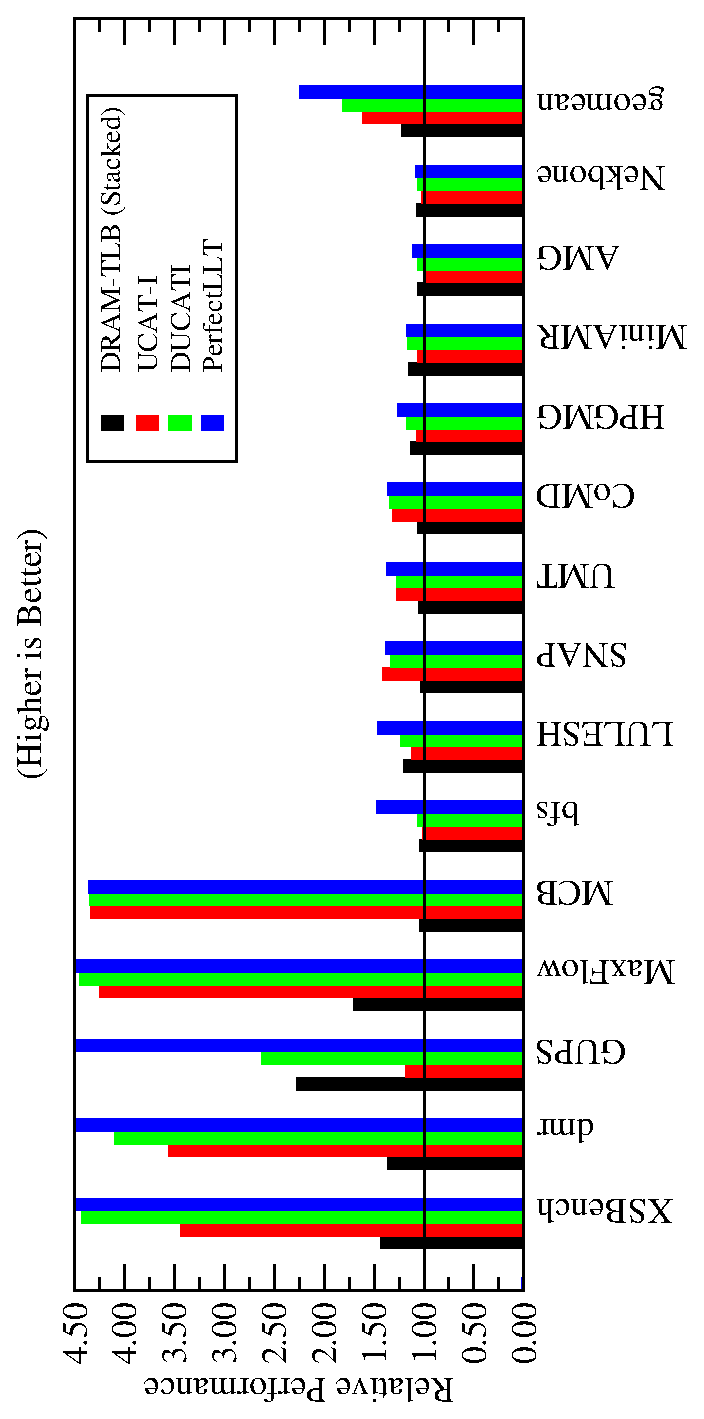
\psfig{file=GRAPHS/SUMMARY_perf,angle=-90,width=\columnwidth}}

\caption{\small Performance Summary (4KB page size).\normalsize}
\label{fig:summary_4k_pages_perf} 
\vspace{0.1 in}
\end{figure}

\begin{figure}[tp] 
\vspace{0.1 in} \centering
\centerline{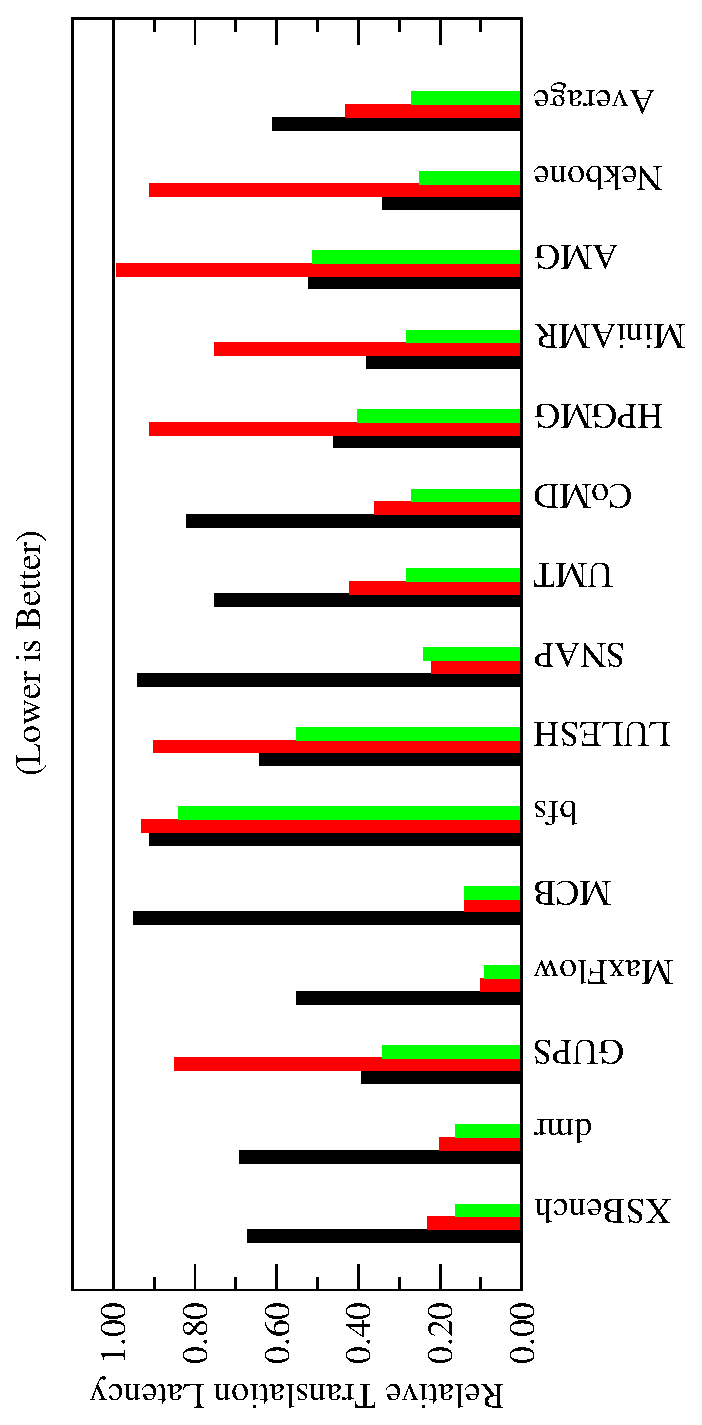
\psfig{file=GRAPHS/SUMMARY_tlblat,angle=-90,width=\columnwidth}}

\caption{\small Translation Latency (4KB page size) (same legend as
  Figure~\ref{fig:summary_4k_pages_perf}).\normalsize}
\label{fig:summary_4k_pages_lat} 
\vspace{-0. in}
\end{figure}

\noindent Figure~\ref{fig:summary_4k_pages_perf} illustrates the
relative performance of our proposals to the baseline system. The
x-axis shows the different workloads while the y-axis illustrates
performance. For each workload, we present the relative performance
for DRAM-TLBs architected with stacked memory (i.e. Stacked-TLB),
Unified Cache and TLB (UCAT) enhanced with insertion (UCAT-I), DUCATI,
and for comparison the unbuildable Perfect Last-Level TLB (LLT)
system. To correlate the reasons for performance improvement,
Figure~\ref{fig:summary_4k_pages_lat} presents the relative address
translation for the different proposals.

Figure~\ref{fig:summary_4k_pages_perf} shows that DRAM-TLBs
architected with stacked memory improves average performance by 22\%,
UCAT with insertion (UCAT-I) improves average performance by 61\%,
while DUCATI combines the benefits of both to improve average
performance by 81\%. These benefits are primarily due to reductions in
the address translation latency. As illustrated in
Figure~\ref{fig:summary_4k_pages_lat}, DUCATI improves address
translation latency by up to 75\%. In doing so, DUCATI bridges 66\% of
the performance gap between the baseline system and a system with a
perfect LLT.



\subsection{DUCATI Sensitivity to Page Size}

\noindent We now present the performance of our schemes using 64KB
page size. For our 1024-entry baseline LLT size, using 64KB pages
increases the TLB coverage to 64MB (up to 256MB because of
~\cite{COLT}). In doing so, the LLT miss frequency reduces for
workloads that have high spatial locality in the virtual address
space. Table~\ref{table:results_summary} summarizes the different
performance metrics relative to the baseline system. With 64KB page
size, Distributed Placement and Stacked-TLB reduce LLT miss latency by
15\% and 39\% respectively. In turn, they improve performance by 4\%
and 12\% respectively.

With 64KB page size, Figure~\ref{fig:summary_64k_pages} presents the
per workload performance behavior of our baseline system, Distributed
Placement and Stacked-TLB relative to a perfect LLT system. We observe
that workloads with high spatial locality within a 64KB page tend to
observe fewer LLT misses. Consequently, the baseline system itself is
within 30\% of a perfect LLT (as opposed to 50\% for the 4KB page size
system). However, there is still opportunity to improve performance of
workloads that are TLB-sensitive with 64KB pages (e.g. $HPGMG$, $DMR$,
and $XSBENCH$). For these workloads, Distributed Placement and
Stacked-TLB proposals improve performance by 27-45\%. Overall,
Stacked-TLB bridges 30\% of the performance gap between the baseline
system and a perfect LLT.


\begin{figure}[tp] 
\vspace{0. in} \centering
\centerline{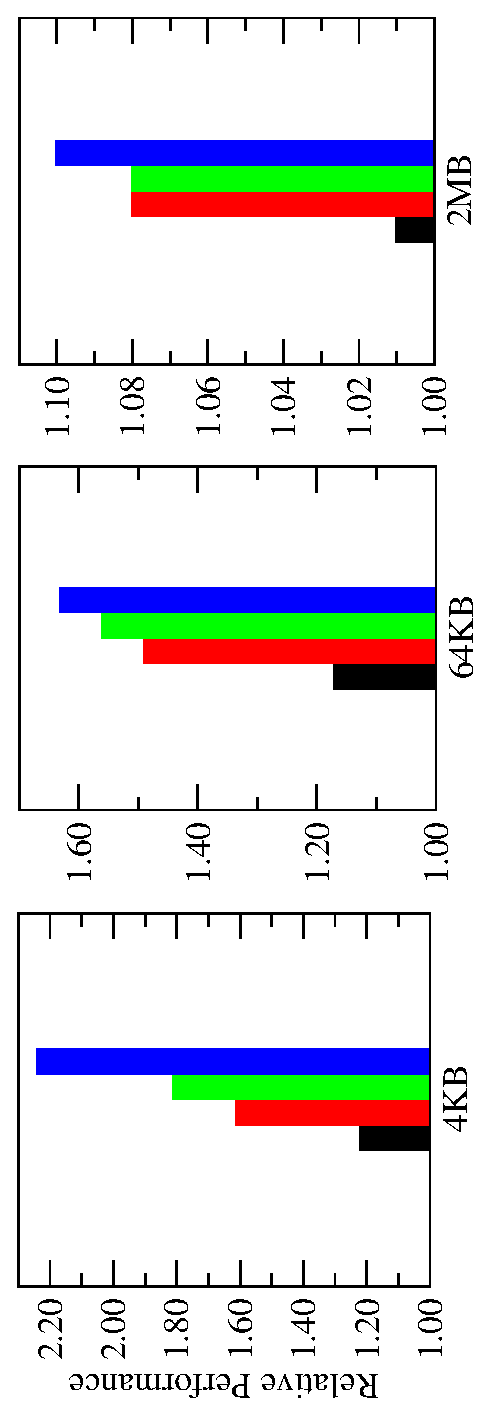
\psfig{file=GRAPHS/pagesize_sensitivity2,angle=-90,width=\columnwidth}}

\caption{\small Performance Sensitivity to Page Size (same legend as
Figure~\ref{fig:summary_4k_pages_perf}). \normalsize}

\label{fig:summary_pagesize} 
\vspace{-0. in}
\end{figure}

% \subsection{Sensitivity to Stacked DRAM Bandwidth}
% 
% \noindent Figure~\ref{fig:stack_bw_sense} illustrates the sensitivity
% of our proposals to stacked memory bandwidth. We evaluate four
% additional systems with 0.25X, 0.5X, 2X, and 4X the stacked memory
% bandwidth of the baseline system (we do not vary the system memory
% bandwidth). We increased the bandwidth by increasing the number of
% channels in the stacked memory system. The y-axis illustrates the
% average performance relative to the baseline system across all
% workloads in the study.
% 
% The figure shows that when the stacked memory bandwidth is plentiful,
% our proposals continue to improve performance. However, when the
% stacked memory bandwidth becomes a bottleneck, the memory queuing
% delays limit the performance of Distributed Placement. Under such
% scenarios, Stacked-TLBs still improve performance since they reduce
% the number of memory references. In general, our proposals efficiently
% utilize the spare bandwidth available in the stacked memory system.
% When the available bandwidth is high, performance improvements are
% high. When the available bandwidth is low, performance improvements
